% R11, 21 September 2026. Requires graphicx in the eventual manuscript.
% The SVG is the vector master; the PNG is for inspection.
% This fragment has not been compiled.
\begin{figure}[ht]
\centering
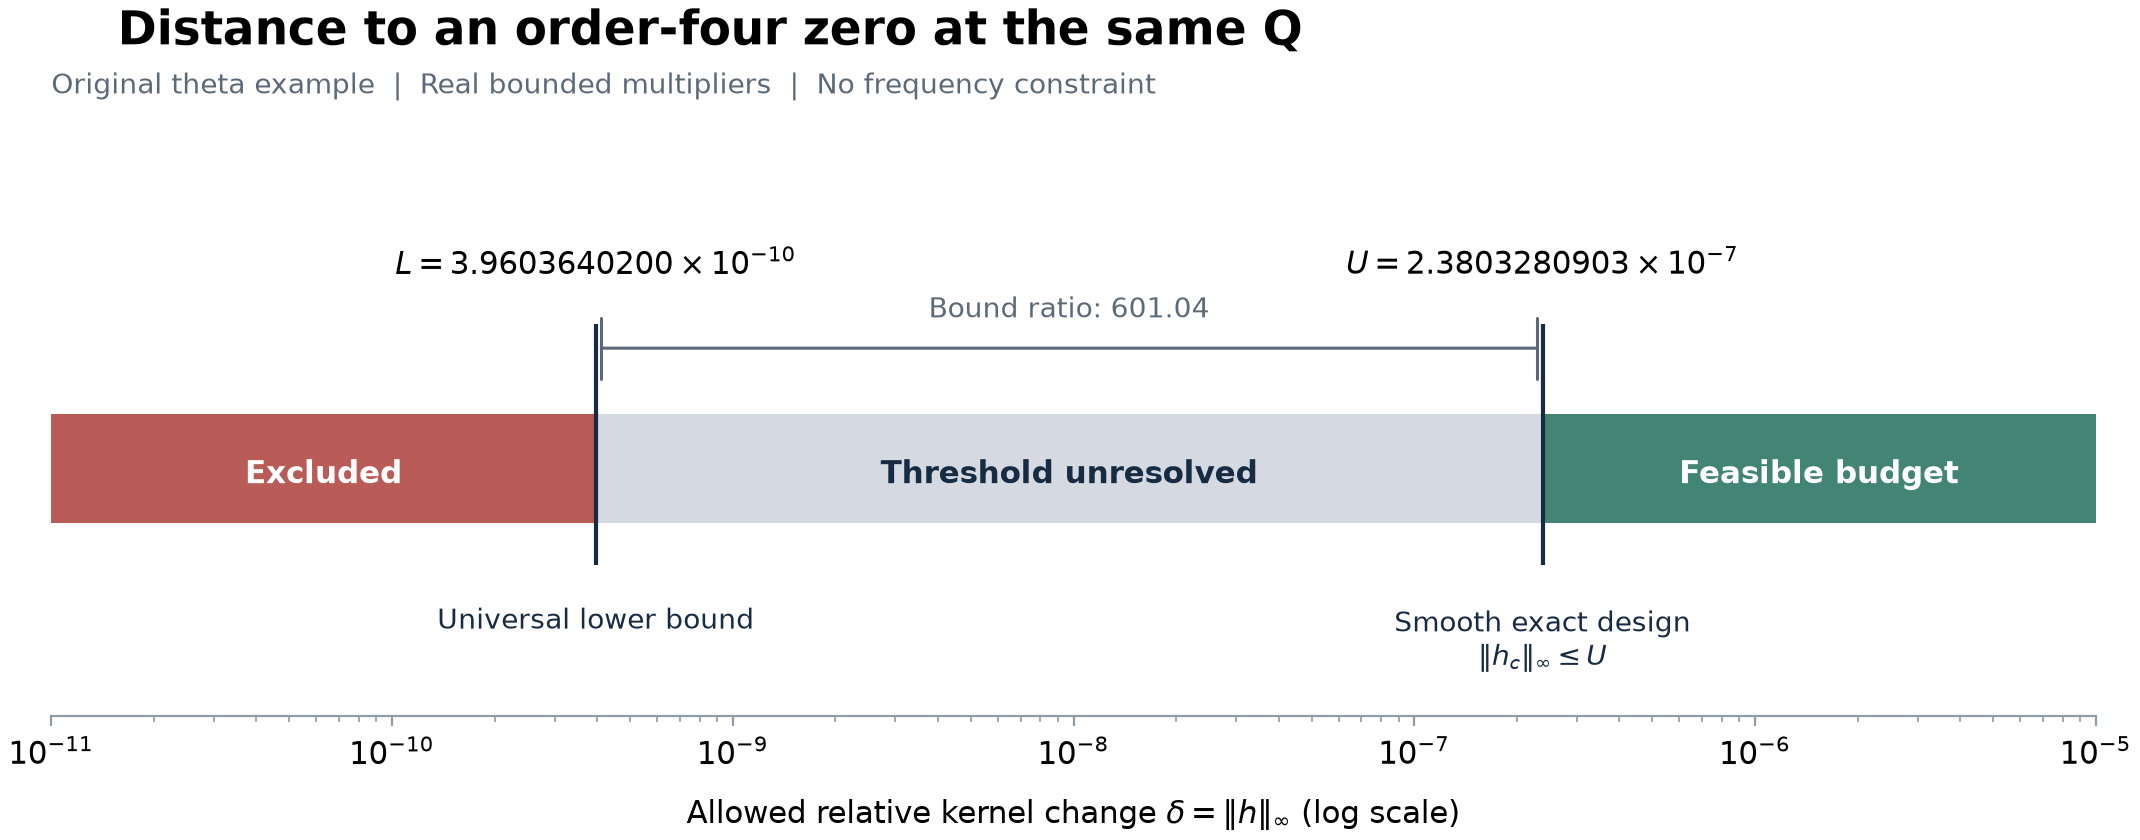
\includegraphics[width=\linewidth]{figures/minimum_relative_change.png}
\caption{First certified bracket on the least relative kernel change
needed to turn the original theta example's order-three zero at the
exact point $Q$ into an order-four zero at the same point. The budget
is $\delta=\|h\|_\infty$ for real bounded multipliers $K(1+h)$, with no
frequency restriction. Budgets below the universal lower bound $L$
are excluded. A smooth nondegenerate design is feasible with norm at
most $U$, so every budget at least $U$ contains that design. The grey
interval leaves the actual threshold unresolved; its bound ratio is
approximately $601.04$. The upper bound uses a coefficient $\ell^1$
sum and need not equal the candidate's supremum norm. The horizontal
axis is logarithmic. This is a budget certificate, not a root-count
map or a plot of a computed optimum.}
\label{fig:r11-cost-bracket}
\end{figure}
